\icode{O-MD-CA-L2-261115-004}
如图所示，质量为\(m_1\) 的木块 \(A\) 和质量为\(m_2\) 的木块\(B\)通过不可伸长的轻绳连接，与地面的摩擦因数均为\(\mu\)。当水平力恒力 \(F_1\)、\(F_2\) 分别作用于左右两端，使\(A\)、\(B\)一起向右加速运动。求\(A\)、\(B\) 间轻绳上的作用力大小。

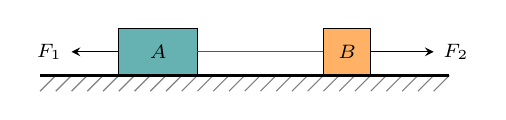
\begin{tikzpicture}[>=stealth,font=\scriptsize]
	\draw[fill=teal!60] (0,0) rectangle(1,0.6)node[midway]{\(A\)};
	\draw[fill=orange!60] (3.2,0) rectangle(2.6,.6)node[midway]{\(B\)};
	\draw[->] (0,.3)--(-.6,.3)node[left]{\(F_1\)};
	\draw[->] (3.2,.3)--(4,.3)node[right]{\(F_2\)};
	\draw[magenta] (1,.3)--(2.6,.3);
	\foreach \x in {-1,-.8,...,4}
		\draw[gray] (\x,-.2)--++(.2,.2);
	\draw[thick] (-1,0)--(4.2,0);
\end{tikzpicture}
\begin{answer}
    
\end{answer}